%%%%%%%%%%%%%%%%%%%%%%%%%%%%%%%%%%%%%%%%%
% Journal Article
% LaTeX Template
% Version 2.0 (February 7, 2023)
%
% This template originates from:
% https://www.LaTeXTemplates.com
%
% Author:
% Vel (vel@latextemplates.com)
%
% License:
% CC BY-NC-SA 4.0 (https://creativecommons.org/licenses/by-nc-sa/4.0/)
%
% NOTE: The bibliography needs to be compiled using the biber engine.
%
%%%%%%%%%%%%%%%%%%%%%%%%%%%%%%%%%%%%%%%%%

%----------------------------------------------------------------------------------------
%	PACKAGES AND OTHER DOCUMENT CONFIGURATIONS
%----------------------------------------------------------------------------------------
\documentclass[
	a4paper, % Paper size, use either a4paper or letterpaper
	10pt, % Default font size, can also use 11pt or 12pt, although this is not recommended
	unnumberedsections, % Comment to enable section numbering
	twoside, % Two side traditional mode where headers and footers change between odd and even pages, comment this option to make them fixed
]{LTJournalArticle}
\usepackage{xcolor}

\addbibresource{sample.bib} % BibLaTeX bibliography file

% \runninghead{Shortened Running Article Title} % A shortened article title to appear in the running head, leave this command empty for no running head

% \footertext{\textit{Journal of Biological Sampling} (2024) 12:533-684} % Text to appear in the footer, leave this command empty for no footer text

\setcounter{page}{1} % The page number of the first page, set this to a higher number if the article is to be part of an issue or larger work

%----------------------------------------------------------------------------------------
%	TITLE SECTION
%----------------------------------------------------------------------------------------

\title{Film Emulation Using Dynamic Range and Tone Mapping} % Article title, use manual lines breaks (\\) to beautify the layout

% Authors are listed in a comma-separated list with superscript numbers indicating affiliations
% \thanks{} is used for any text that should be placed in a footnote on the first page, such as the corresponding author's email, journal acceptance dates, a copyright/license notice, keywords, etc
\author{%
	Christian Johnson\textsuperscript{1}, Alex Martin\textsuperscript{2} 
}

% Affiliations are output in the \date{} command
\date{\footnotesize\textsuperscript{\textbf{1}}Harvey Mudd College, \texttt{chrjohnson@hmc.edu} \\ \textsuperscript{\textbf{2}}Harvey Mudd College, \texttt{almartin@hmc.edu}}

% % Full-width abstract
% \renewcommand{\maketitlehookd}{%
% 	\begin{abstract}
% 		\noindent Lorem ipsum dolor sit amet, consectetur adipiscing elit. Praesent porttitor arcu luctus, imperdiet urna iaculis, mattis eros. Pellentesque iaculis odio vel nisl ullamcorper, nec faucibus ipsum molestie. Sed dictum nisl non aliquet porttitor. Etiam vulputate arcu dignissim, finibus sem et, viverra nisl. Aenean luctus congue massa, ut laoreet metus ornare in. Nunc fermentum nisi imperdiet lectus tincidunt vestibulum at ac elit. Nulla mattis nisl eu malesuada suscipit. Aliquam arcu turpis, ultrices sed luctus ac, vehicula id metus. Morbi eu feugiat velit, et tempus augue. Proin ac mattis tortor. Donec tincidunt, ante rhoncus luctus semper, arcu lorem lobortis justo, nec convallis ante quam quis lectus. Aenean tincidunt sodales massa, et hendrerit tellus mattis ac. Sed non pretium nibh. Donec cursus maximus luctus. Vivamus lobortis eros et massa porta porttitor.
% 	\end{abstract}
% }

%----------------------------------------------------------------------------------------

\begin{document}

\maketitle % Output the title section

%----------------------------------------------------------------------------------------
%	ARTICLE CONTENTS
%----------------------------------------------------------------------------------------

\section{Introduction}

With the increasing affordability of technology [1] and the widespread use of smartphones [2], nearly everyone now has access to a camera. This has opened up new possibilities for capturing and sharing images, but it also presents challenges. When taking an image with a camera, the range of light and dark values it can represent at once is its dynamic range, with values outside of this range being completely dark or completely light, thus possessing no visual information. Dynamic range is a central challenge in computational photography and image processing, as scenes with a wide range of light and dark become difficult to effectively capture and represent. 

High dynamic range (HDR) photography is a popular solution for addressing dynamic range limitations. There are many approaches to creating an HDR image, with Deep Learning becoming an increasingly popular area [3], but the most widely used approach is image composition. In this method multiple images of the same scene are taken at different exposures, and then digitally combined to create a single image where areas of under/over exposure are filled in by the full set of images.

The result, however, is not yet a compelling photograph. Most displays and printing mediums are not designed for HDR images, and thus the wide range of exposure information will make the image seem low-contrast and dull. To correct this a technique called tone mapping is used, in which an HDR image is normalized and adjusted to match the contrast needs of displays while preserving the details and balance developed in the composite. Tone mapping is a critical step in making HDR imaging practical, as it enables HDR images to be viewed on standard displays. 

This project aims to integrate image registration techniques for HDR composition with tone mapping methods designed to emulate the aesthetic qualities of film photography. The combination of the technical and artistic aspects represents a unique approach to HDR imaging. 

%------------------------------------------------

\section{Related Work}

The core approach of our project is to make use of the Debevec algorithm (also known as the Debevec-Malik algorithm). The Debevec algorithm pioneered HDR compositing, and remains to be widely used in computer vision projects requiring HDR image handling, with the original paper receiving over 4000 citations. Given its long standing popularity and effective results, our project ultimately sought to re-implement the Debevec algorithm in a complete pipeline to generate compelling images of high-contrast scenes. 

The algorithm, first published in SIGGRAPH ‘97 was actually designed with the intent of producing high-quality digitizations of film scans. Most available scanning technology at the time of this paper’s writing had a dynamic range more limited than that of most film stocks, and thus digitizing images from film would result in a loss in image quality. While our project focuses on a different application of HDR compositing, this methodology will still work, although some care will need to be taken to ensure that the images are prepared properly. In particular, images will need to be registered such that pixel values for each exposure align to the same relative points in the image.

The Debevec algorithm works by leveraging image reciprocity to generate a representation of the full light -or radiance- of the scene. Reciprocity is the relationship in which the brightness of a given point on a photograph (pixel value for digital cameras, or density for film images) is the result of the radiance of the corresponding area of the scene and the exposure settings regulating the amount of light, modulated by the medium’s response function. The response function is a property of imaging systems where cameras respond less to extremely bright or dark regions, and respond more to more neutral areas of the image. Thus, since the brightness of each pixel and settings for each exposure are known, the Debevec algorithm uses the reciprocity relationship to calculate the camera response function for the image. Once the camera response function is created, an HDR radiance map can be generated by taking each pixel value and using the response function to calculate the radiance for that pixel. The result is an HDR representation of the full range of light (as can be captured from the given exposure range) for the scene.

Thus, our project uses this algorithm to generate a radiance map, from which a tone mapping function can be used to convert the map to a compelling image with a natural amount of contrast.


\section{Methodology}

\subsection{Dataset}
After evaluating existing datasets and finding none that met the specified requirements of our HDR task, we decided to create a custom dataset tailored to our project [1]. The data set consists of thirteen sets of images captured around the academic end of Harvey Mudd’s campus. 

To ensure minimal movement between shots, we used a tripod and a \textbf{[Alex’s Camera name (I think Sony A7)]} camera. At each location, we captured several images of the same scene while systematically varying the exposure levels. The exposure times ranged from 1/8000th of a second to 1/30th of a second, providing a broad spectrum of lighting conditions to support HDR image composition and tone mapping.  
	% \textbf{[Add about converting raw files to file format usable for openCV]}

\subsection{Image Registration}
Despite using a tripod to minimize displacement between images, there was still a noticeable amount of movement between successive shots, necessitating image registration. The goal of image registration was to align all images captured for the same scene to a single reference image, ensuring alignment for HDR processing.
For each scene, we selected a reference image that served as the "ground truth." The remaining images were aligned to this reference image using the following steps:

Key Points were detected in both the reference image and the other images using the AKAZE feature detection algorithm. This choice was made for its efficiency and robustness in capturing distinctive features [1]. The detected features were matched between the reference image and each other image using a brute force matcher with Hamming distance as the metric. To ensure quality matches, we kept the top 75\% of matches or at least 10 matches, whichever was greater. Using the matched features, a homography transformation matrix was computed with the RANSAC algorithm. This matrix encapsulated the transformation required to align each image with the reference image. Each image was warped using the computed transformation matrix, aligning it to the reference image. Warping was necessary due to perspective distortions caused by lens or viewpoint differences. 

After alignment, residual black borders were present in some images due to the warping process. To eliminate these artifacts, we determined the minimum bounding box that encompassed all valid image regions across the aligned images. The images were then cropped to this bounding box, ensuring uniformity across the dataset and avoiding artifacts in the HDR computation. This process produced a set of images that were fully aligned and ready for HDR composition.

\subsection{Debevec Algorithm}
While OpenCV does contain a set of functions to run the Debevec algorithm, in our testing we found the results of these functions to be questionable, oftentimes incorrectly compositing different exposures in a manner that was not accurate to the scene. Thus, we decided to implement the Debevec algorithm from scratch as described in the paper. This implementation of HDR compositing works in the following steps:
\begin{itemize}
	\item Randomly select sample pixels from the image to generate the response function – in our testing 100 samples worked well.
	\item Collect the values of each sample pixel independently for each color channel, as the algorithm is designed for monochrome processing.
	\item Run the objective function O (Equation 3) on each of the three sets of samples to calculate the response function. This implementation was made easy by copying the Matlab code provided in the paper.
	\begin{itemize}
		\item This function makes use of a secondary weighting function that was also implemented. A number of weighting functions are possible, but we implemented the function described in Equation 4 that emphasizes smoothness in the center of the curve. This results in a very reasonable response curve output.
	\end{itemize}
	\item Run Equation 6 for each pixel in the image to calculate the radiance for every position, using the same weighting function to give priority to values in the middle exposure range that have more image sensitivity.
\end{itemize}
The result of these steps is a radiance map that after tone mapping exhibits the desired properties of a successful HDR composite. While the equations were pulled directly from the paper, it took some work to translate the Matlab code for function O and implement equations 4 and 6. Likewise, the resulting process is quite slow, especially on larger images due to the pixel-wise iteration. However, it worked much more consistently and effectively for our purposes than the OpenCV implementation, and thus we selected this approach for our code.

\subsection{Reinhard Tone Mapping}
Running the Debevec algorithm over the images of varying exposure allows us to capture a wide range of values. However, this resulting HDR image has pixel values that exceed the dynamic range of standard display devices. Thus, tone mapping is required to compress the high dynamic range of an HDR image while ensuring the image remains visually compelling. 

We chose to use Reinhard as our tone mapping operator which we implemented as directed in Reinhard's paper [1]. First, the log-average luminance of the scene is calculated using the following formula where $N$ is the number of pixels, delta is a small value to avoid the logarithm of zero and $L_w$ are the values from the HDR image.

\begin{equation}
	\overline{L}_w = \frac{1}{N} \exp\left( \sum_{x,y} \log(\delta + L_w(x,y))\right)
\end{equation}

After the log-average luminance is calculated, the HDR image values are normalized over the log-average luminance previously calculated. This normalization scales the scene to a middle-gray value, $\alpha$, which controls the scene's brightness. 

\begin{equation}
	L(x,y) = \frac{\alpha}{\overline{L}_2} L_w(x,y)
\end{equation}

Finally, we used the normalized values to calculate the resulting image values. For our implementation, we chose the extended Reinhard operator:

\begin{equation}
	L_d(x,y) = \frac{L(x,y)(1 + \frac{L(x,y)}{L^2_{white}})}{1 + L(x,y)}
\end{equation}

Unlike the basic Reinhard operator this equation allows precise control over which values are mapped to white. For our implementation we determined the $L_{white}$ value based on the maximum luminance from equation 2. This tone mapping process transforms our HDR output from the Debevec algorithm into a visually appealing image which can be displayed on standard devices.

While Reinhard’s paper provided us with a conceptual understanding of the tone mapping we also referenced Deepan’s github repository [2] for the practical implementation of the Reinhard operator.

\subsection{Artificial Bloom}

To help our tonemapped HDR image feel more natural, we finished the image by adding a slight “blooming” effect to the highlights. This works by selecting the pixels above a chosen brightness threshold to make a mask, and then blurring the mask to cover a wider area with a gradient. From there we can boost the brightness of the image based on the area of the mask, giving a blooming effect in which brightly exposed areas bleed over to darker areas, mimicking both the human visual system and a common property of photographic films. The resulting effect provides an interesting stylistic look to the image that allows for the high dynamic range of the image to feel more natural by giving the impression that brighter areas are in fact brighter than they really are.

We finally finish the image through a basic white balancing algorithm – the gray world algorithm, that centers each color channel to a median value for the image to compensate for channel variation that could occur from the individual response function calculation.


%------------------------------------------------

% \section{Results}

% \begin{table} % Single column table
% 	\caption{Example single column table.}
% 	\centering
% 	\begin{tabular}{l l r}
% 		\toprule
% 		\multicolumn{2}{c}{Location} \\
% 		\cmidrule(r){1-2}
% 		East Distance & West Distance & Count \\
% 		\midrule
% 		100km & 200km & 422 \\
% 		350km & 1000km & 1833 \\
% 		600km & 1200km & 890 \\
% 		\bottomrule
% 	\end{tabular}
% 	\label{tab:distcounts}
% \end{table}

% Referencing a table using its label: Table \ref{tab:distcounts}.

% \begin{table*} % Full width table (notice the starred environment)
% 	\caption{Example two column table with fixed-width columns.}
% 	\centering % Horizontally center the table
% 	\begin{tabular}{L{0.2\linewidth} L{0.2\linewidth} R{0.15\linewidth}} % Manually specify column alignments with L{}, R{} or C{} and widths as a fixed amount, usually as a proportion of \linewidth
% 		\toprule
% 		\multicolumn{2}{c}{Location} \\
% 		\cmidrule(r){1-2}
% 		East Distance & West Distance & Count \\
% 		\midrule
% 		100km & 200km & 422 \\
% 		350km & 1000km & 1833 \\
% 		600km & 1200km & 890 \\
% 		\bottomrule
% 	\end{tabular}
% \end{table*}

% Aenean feugiat pellentesque venenatis. Sed faucibus tristique tortor vel ultrices. Donec consequat tellus sapien. Nam bibendum urna mauris, eget sagittis justo gravida vel. Mauris nisi lacus, malesuada sit amet neque ut, venenatis tempor orci. Curabitur feugiat sagittis molestie. Duis euismod arcu vitae quam scelerisque facilisis. Praesent volutpat eleifend tortor, in malesuada dui egestas id. Donec finibus ac risus sed pellentesque. Donec malesuada non magna nec feugiat. Mauris eget nibh nec orci congue porttitor vitae eu erat. Sed commodo ipsum ipsum, in elementum neque gravida euismod. Cras mi lacus, pulvinar ut sapien ut, rutrum sagittis dui. Donec non est a metus varius finibus. Pellentesque rutrum pellentesque ligula, vitae accumsan nulla hendrerit ut.

% \begin{figure} % Single column figure
% 	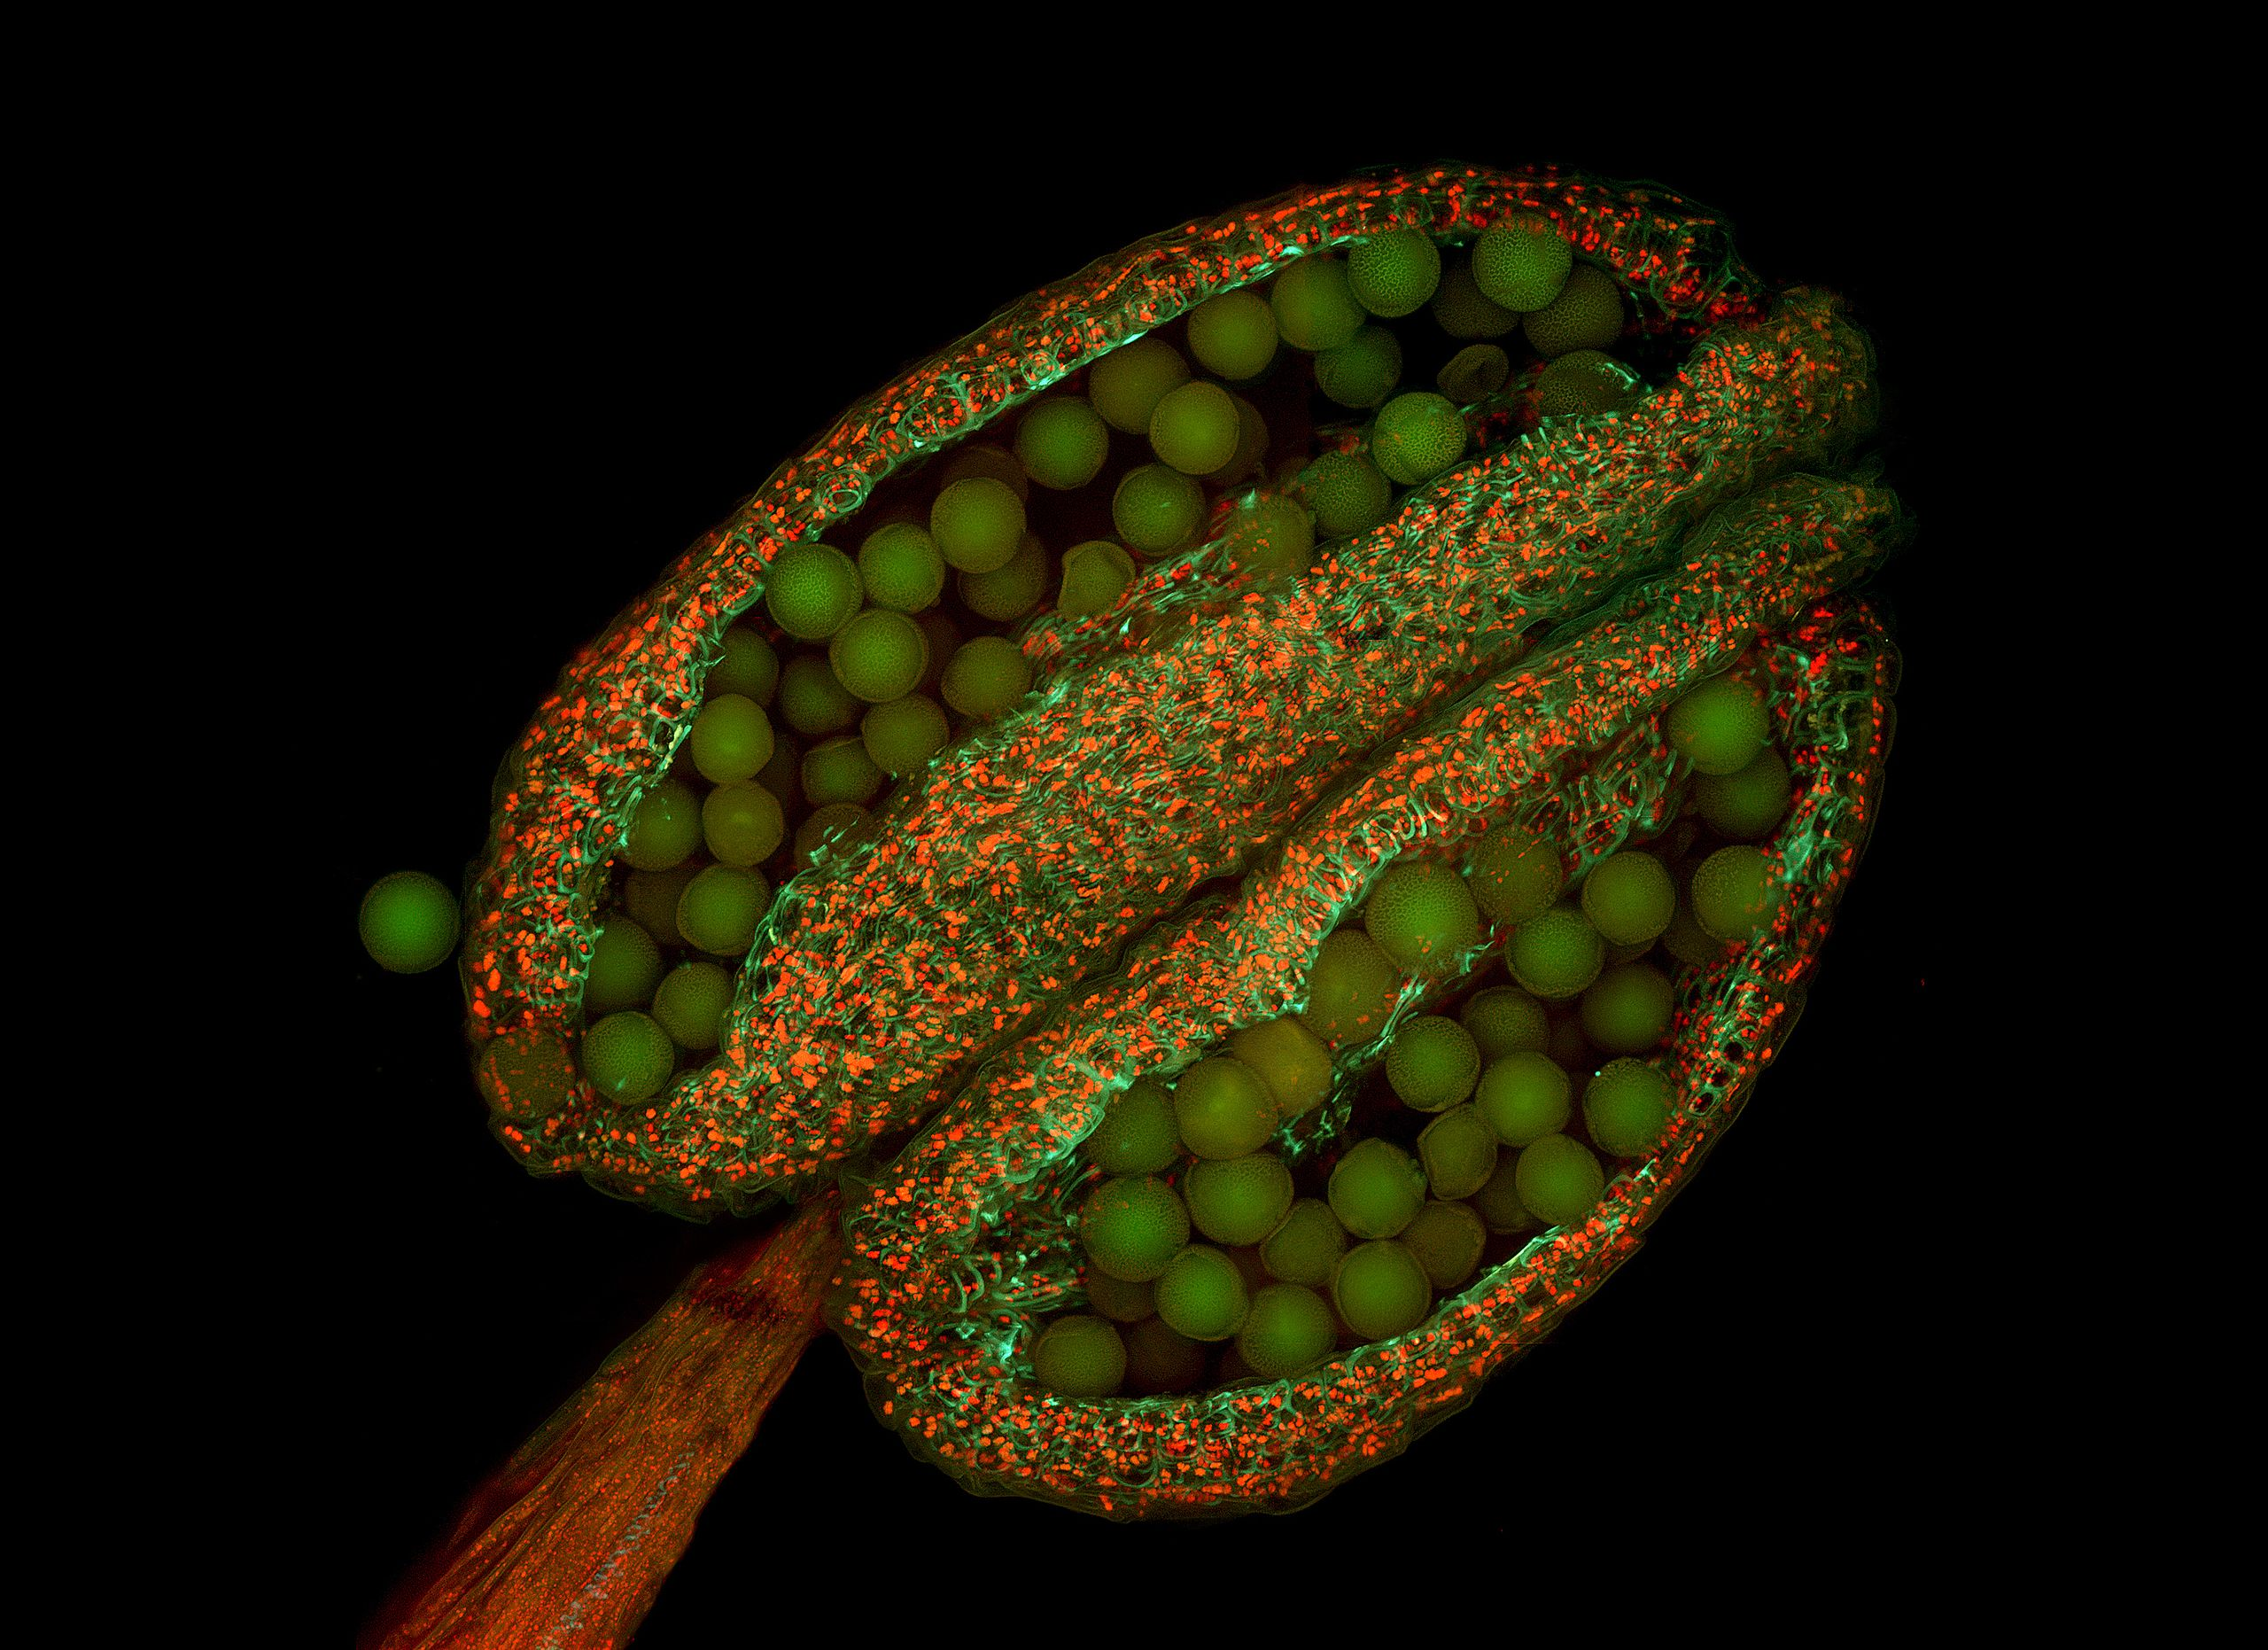
\includegraphics[width=\linewidth]{Tolmukapea.jpg}
% 	\caption{Anther of thale cress (Arabidopsis thaliana), fluorescence micrograph. Source: Heiti Paves, \href{https://commons.wikimedia.org/wiki/File:Tolmukapea.jpg}{https://commons.wiki-\\media.org/wiki/File:Tolmukapea.jpg}.}
% 	\label{fig:tcanther}
% \end{figure}

% Referencing a figure using its label: Figure \ref{fig:tcanther}.

% Aenean porttitor eros non pharetra congue. Proin in odio in dolor luctus auctor ac et mi. Etiam euismod mi sed lectus fringilla pretium. Phasellus tristique maximus lectus et sodales. Mauris feugiat ligula quis semper luctus. Nam sit amet felis sed leo fermentum aliquet. Mauris arcu dui, posuere id sem eget, cursus pulvinar mi. Donec nec lacus non lectus fermentum scelerisque et at nibh. Sed tristique, metus ac vestibulum porta, tortor lectus placerat lorem, et convallis tellus dolor eget ante. Pellentesque dui ligula, hendrerit a purus et, volutpat tempor lectus. Mauris nec purus nec mauris rhoncus pellentesque. Quisque quis diam sed est lacinia congue. Donec magna est, hendrerit sed metus vel, accumsan rutrum nibh.

% \begin{figure*} % Two column figure (notice the starred environment)
% 	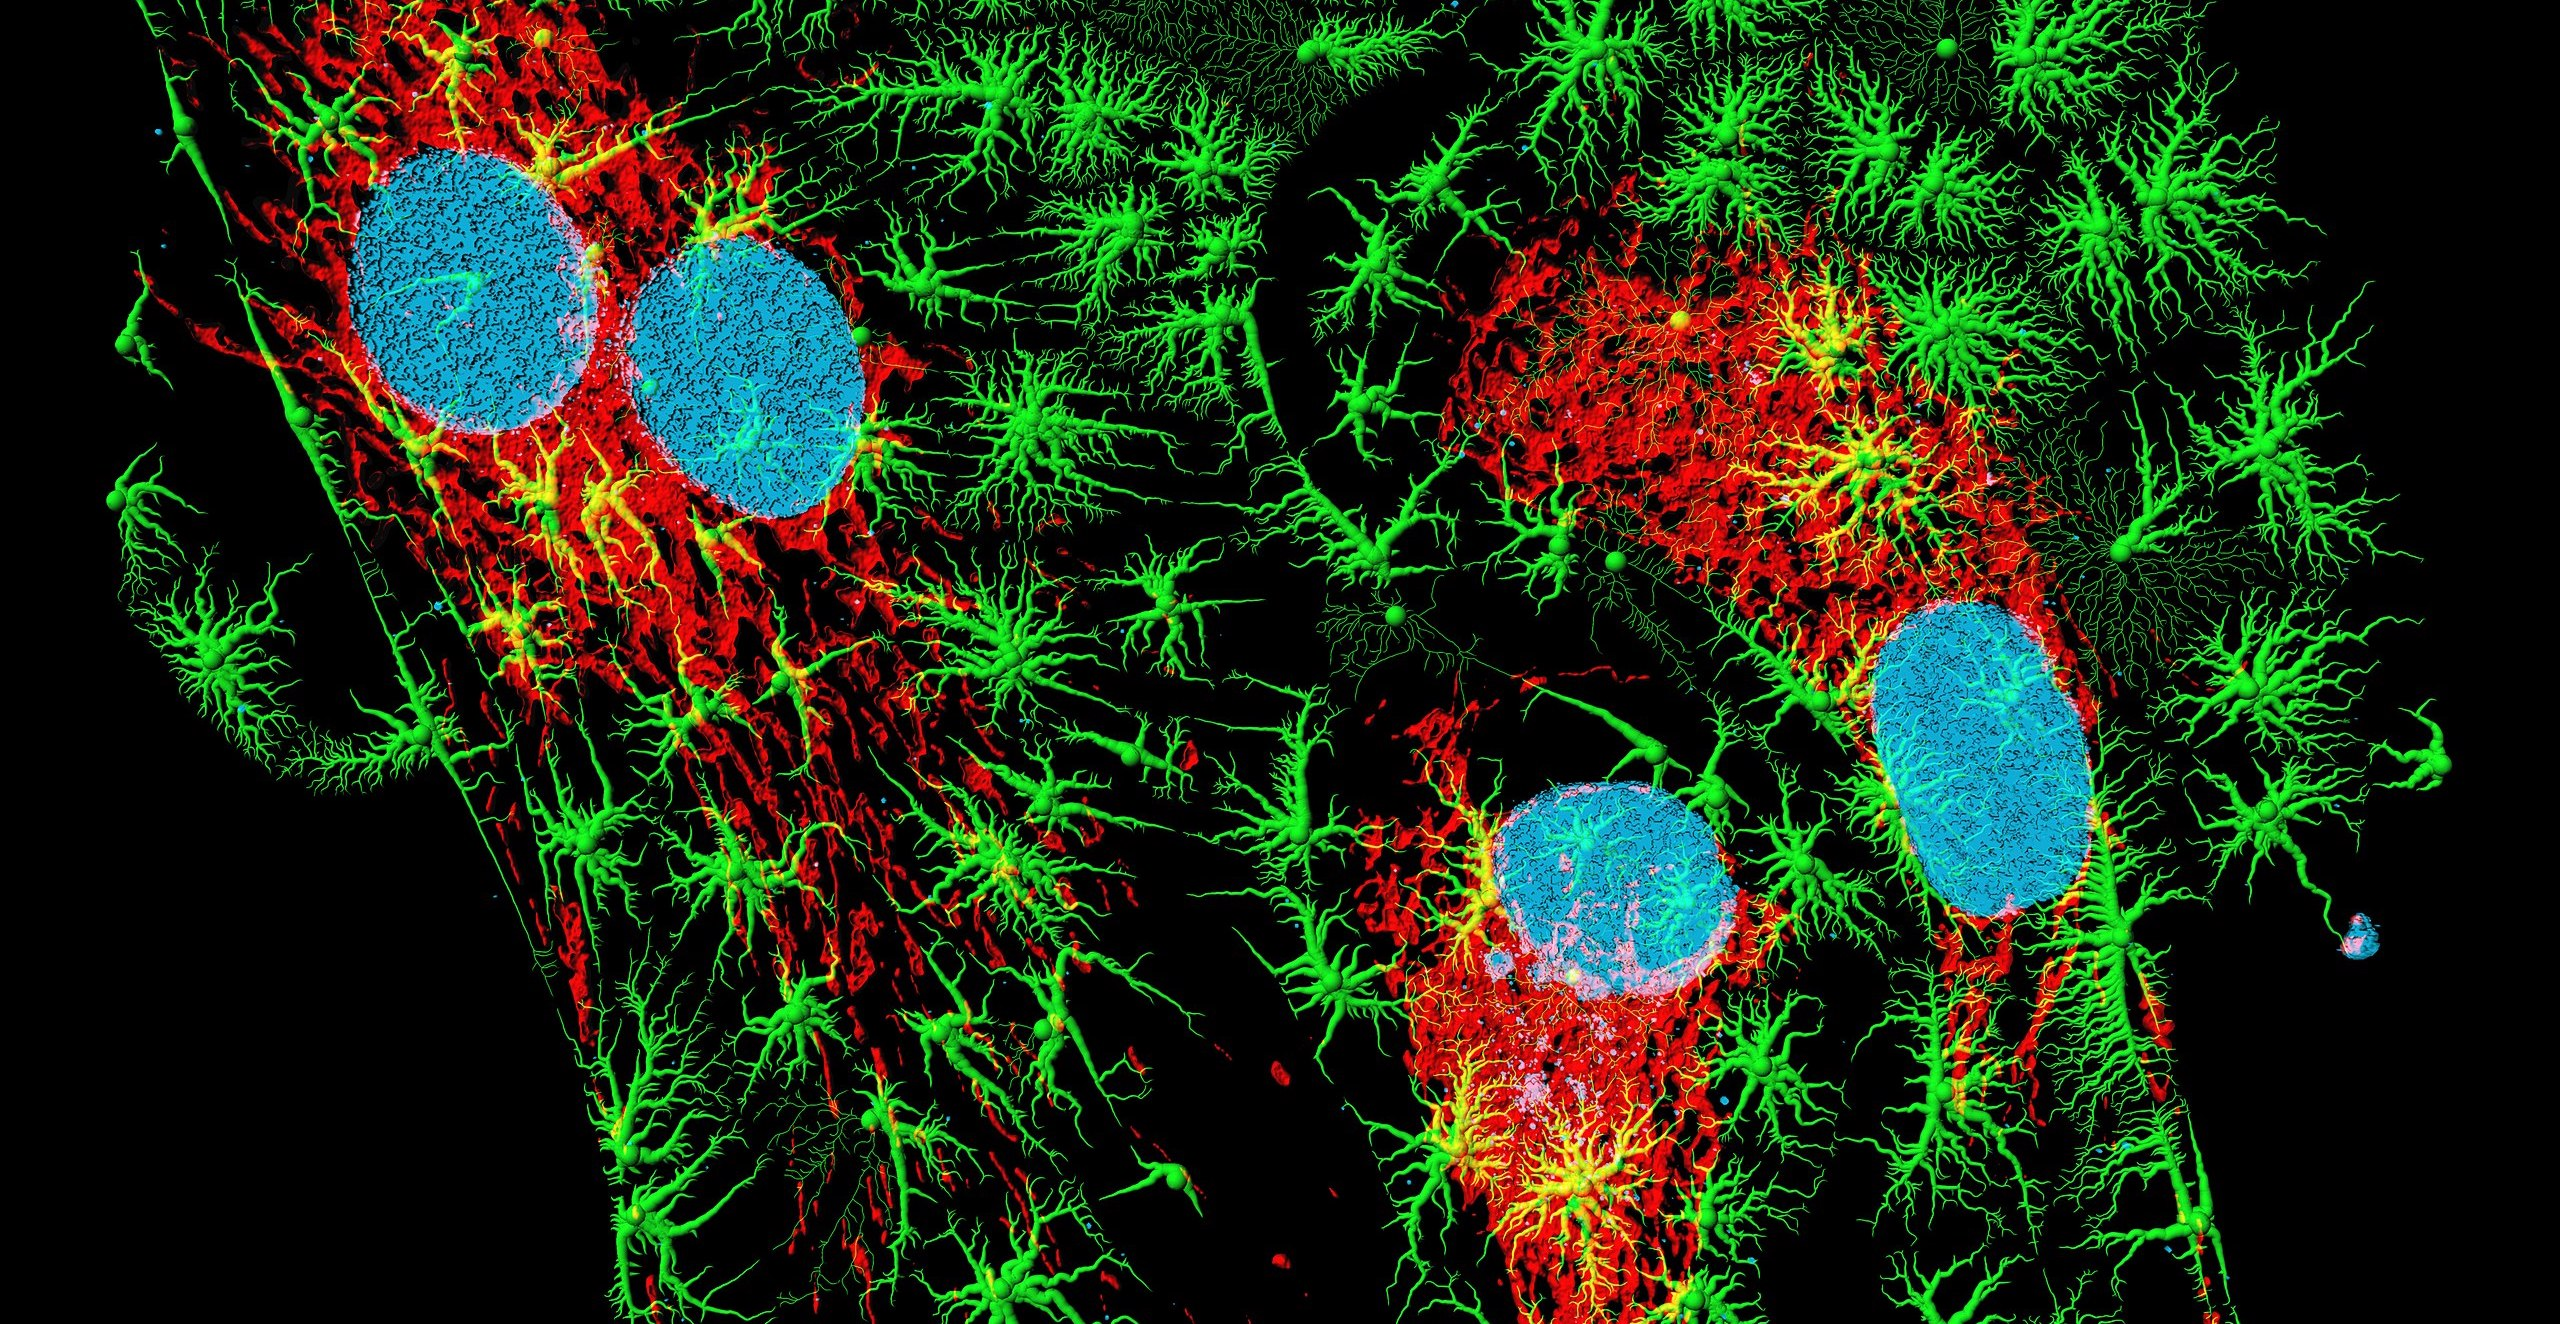
\includegraphics[width=\linewidth]{Fibroblastid.jpg}
% 	\caption{Bovine pulmonary artery endothelial cells in culture. Blue: nuclei; red: mitochondria; green: microfilaments. Computer generated image from a 3D model based on a confocal laser scanning microscopy using fluorescent marker dyes. Source: Heiti Paves, \href{https://commons.wikimedia.org/wiki/File:Fibroblastid.jpg}{https://commons.wikimedia.org/wiki/File:Fibroblastid.jpg}.}
% 	\label{fig:bpartery}
% \end{figure*}

% Orci varius natoque penatibus et magnis dis parturient montes, nascetur ridiculus mus. Etiam cursus lectus purus, tempus iaculis quam dictum tristique. Nam interdum sapien nec tempor mattis. Quisque id sapien nisi. Mauris vehicula ornare eros vel efficitur. Nulla consectetur, turpis quis fringilla tincidunt, mi neque iaculis lectus, vel commodo elit odio non ex. Duis facilisis, purus ac viverra iaculis, turpis lectus ultrices ante, ac vestibulum ligula magna in libero. Etiam tristique maximus lacinia. Vestibulum hendrerit, lacus malesuada laoreet blandit, sapien velit sollicitudin nunc, eu porttitor urna ligula at lorem. Aliquam faucibus eros in fermentum venenatis. Fusce consectetur congue pellentesque. Suspendisse at nisi sit amet est porttitor cursus. Cras placerat faucibus nunc, a laoreet justo dignissim sit amet.

% \subsection{International Support}

% \noindent àáâäãåèéêëìíîïòóôöõøùúûüÿýñçčšž

% \noindent ÀÁÂÄÃÅÈÉÊËÌÍÎÏÒÓÔÖÕØÙÚÛÜŸÝÑ

% \noindent ßÇŒÆČŠŽ

% \subsection{Links}

% This is a clickable URL link: \href{https://www.latextemplates.com}{LaTeX Templates}. This is a clickable email link: \href{mailto:vel@latextemplates.com}{vel@latextemplates.com}. This is a clickable monospaced URL link: \url{https://www.LaTeXTemplates.com}.

% %------------------------------------------------

\section{Results}
For each of the thirteen scenes in our data set of images around the Harvey Mudd campus, we ran the Debevec algorithm, Reinhard tone mapping operator and bloom effects. This produced a camera response function graph with a corresponding HDR image of the scene. The images and camera response functions can be found on \underline{\textcolor{blue}{\href{https://drive.google.com/drive/folders/1Jsv7LVcdsvOUPuSliDZ4YODO_5oRG9gu?usp=share_link}{Google Drive}}}.

\subsection{Qualitative Evaluation}
For scenes with both bright outdoor areas and dark shadowed regions, our pipeline successfully retained details in both extremes. For example, in the eighth scene where a single shot from a digital camera would either blow out the sky or lose detail in shadowed areas, our HDR reconstruction maintains detail throughout the entire scene.

In addition, the Reinhard tone mapping preserved a natural looking color reproduction while compressing the dynamic range of the HDR image. This is particularly evident in scene nine with the colorful flowers under varying light conditions.

Overall, the final tone-mapped images combined with the bloom and white balance techniques exhibit a balanced, natural appearance without the image looking artificial as some “HDR” implementations suffer from.

One shortcoming of our implementation is in scenes in which objects had displacement between shots. For example, in scene eight the tree branches were swaying due to wind and in scene six the water spouting from the fountain. The movement between shots in these scenes resulted in a ghosting effect.


\textbf{This statement requires citation \autocite{Smith:2023qr}. This statement requires multiple citations \autocite{Smith:2023qr, Smith:2024jd}. This statement contains an in-text citation, for directly referring to a citation like so: \textcite{Smith:2024jd}.}

\subsection{Quantitative Evaluation}

While we initially planned on using functions implemented in OpenCV’s library the outputs of OpenCV’s Debevec function looks unnatural. Therefore, we decided to hand implement the Debevec algorithm along with the Reinhard tone mapping operator.

While our implementation of the Debevec algorithm resulted in better looking images the run time suffered. The functions of our code associated with the Debevec algorithm took up to 10 minutes to process nine images. This was far slower than OpenCV’s implementation of the Debevec algorithm.  

The camera response function recovered through our implementation offers valuable insights to both our pipeline’s effectiveness and the characteristics of the camera we used. The curve characteristics, color channel comparison, and consistency across give us metrics to evaluate the camera response functions. 

The camera response functions recovered throughout our implementation consistently display the expected S-curve shape characteristic of digital cameras. Each function exhibits a relatively linear central region with compressed responses in both the low and high intensity areas which accurately reflects how digital sensors translate light intensity to pixel values [1]. We observed smooth, monotonically increasing curves across all recovered functions which validates Debevec algorithm implementation. 

Visual inspection of the camera response functions from all thirteen scenes reveals a high consistency. The curves maintain nearly identical shapes and minimal separations between corresponding channels. While the majority of response functions were consistent across scenes there did exist some outlier curves that, although maintaining the S-shape and inflection points, exhibited increased noise. The most major outlier was scene twelve which featured more extreme lighting conditions. Despite this increased noise, the shape of the curves remained relatively consistent with the other response functions.



\section{Conclusion}

We were able to create a data set of images and implement a pipeline to process a series of digital images, varying in exposure, to create a HDR image encapsulating the aesthetic found in film images. 

While successful in our task there are some areas in our project which could be developed further in the future. Given the current computational inefficiencies in our implementation of the Debevec algorithm we could look at OpenCV’s implementation to make the run time faster. 
As mentioned in the results section scenes with even slight motion resulted in ghosting in the final image. There has been research done [1] to remedy the ghosting issue and a future work could involve implementing these deghosting algorithms to create a more clear final product.


%----------------------------------------------------------------------------------------
%	 REFERENCES
%----------------------------------------------------------------------------------------

\printbibliography % Output the bibliography

%----------------------------------------------------------------------------------------

\end{document}
